\section{Vorgehen}
\subsection{Vorgehensmodell}
Wir haben uns nach Absprache mit unserem Betreuer Professor Matthias Hirth für ein agiles Vorgehensmodell entschieden. Durch den engen Kontakt zu den Auftraggebern ist davon auszugehen, dass sich während der Entwicklung der Software Änderungen an den anfänglich vorgegebnen Anforderungen ergeben. Um möglichst viel Flexibilität zu gewährleisten, bietet sich eine durch Prototypen getriebene Entwicklung an. Die weitergehenden Anforderungen werden im Laufe des Projekts in den Gesprächen mit den Auftraggebern entwickelt. \par
\vspace{0,5cm}
\noindent Als Vorgehensmodell orientieren wir uns an einer auf Agilität angepassten Version des Unified Prozess, wie in Abbildung \ref{fig:UPAgil} dargestellt. Dieses Vorgehen harmoniert gut mit der Aufteilung des Softwareprojekts in Phasen, da in 3 Iterationen entwickelt wird.

\begin{figure}[htp]
    \centering
    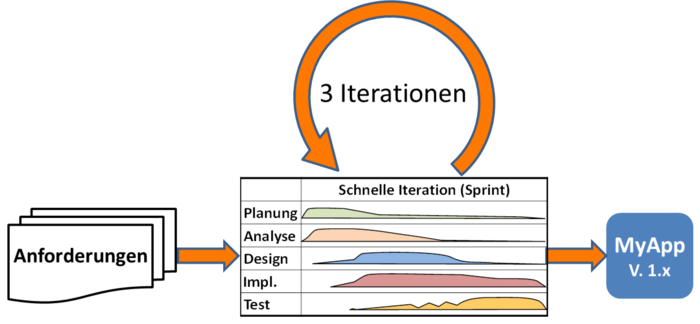
\includegraphics[width=14cm , height=7cm]{Kapitel/Bilder/AgileUnifiedProcess.png}
    \caption[Schema des Vorgehensmodells]{Schema des Vorgehensmodells\protect\footnotemark}
    \label{fig:UPAgil}
\end{figure}
\footnotetext{https://www.tu-ilmenau.de/sse/lehre/softwareprojekt/projektablauf/\#jfmulticontent\_c196637-3, abgerufen am 12.05.2020}

\newpage

\subsection{Alternativen}
\noindent Scrum sowie ExtremeProgramming erscheinen aufgrund der begrenzten Erfahrung des Teams nicht geeignet. Außerdem kann, um das volle Potenzial dieser Verfahren auszuschöpfen, nicht ausreichend Wochenarbeitszeit investiert werden.

\vspace{1,5cm}

\subsection{Durchführung}
\noindent Um einen entwicklungsgetriebenen Ablauf zu gewährleisten arbeiten wir die Projektphasen stark überlappend ab. Vor allem die Phasen "`Analyse"', "`Design"' und "`Implementierung"' werden bei der Entwicklung des Prototypen gleichzeitig ausgeführt. Die entwickelten Anforderungen werden inkrementell implementiert. Aus den gemachten Erfahrungen ergeben sich teils sofort, teils für die weitere Entwicklung, Änderungen. Nach der Implementierung einer Anforderung werden sie in ersten Tests auf ihre Funktionalität überprüft und entsprechende Fehler sofort behoben.

\noindent Ziel der ersten Iteration ist es einen Überblick über Aufwand, Technologie und Risiken zu gewinnen sowie einen lauffähigen Prototypen zu entwickeln. Die Planung der zweiten Iteration basiert auf den Erfahrungen mit dem ersten Prototypen und beginnt nach Präsentation der Ergebnisse der ersten Iteration.

\newpage

\subsection{Werte und Prinzipien}
\vspace{1cm}
\subsubsection*{Werte}

\begin{itemize}
    \item Wir sind als Mitglieder gleichberechtigt und verpflichtet zur Mitarbeit am Projekt.
    \item Wir bringen uns gegenseitigen Respekt und Wertschätzung entgegen.
    \item Wir leben eine offene Kommunikation und Fehlerkultur.
    \item Wir bieten uns gegenseitige Hilfe und Unterstützung an.
\end{itemize}{}

\subsubsection*{Prinzipien}
\begin{itemize}
    \item KISS
    \item Wir halten den Code ständig lauffähig.
    \item Wir arbeiten gemeinsam im Pair-Programming.
    \item Wir machen keine Überstunden.
\end{itemize}{}
